% !TEX root = ../main.tex
\chapter{Resultados y análisis}\label{cap:evaluacion}

Este capítulo presenta el análisis cuantitativo y cualitativo de los resultados obtenidos en cada caso de uso, discute las diferencias de rendimiento entre algoritmos cuánticos y clásicos a la luz del estado del arte, y evalúa las implicaciones prácticas para su aplicación en el contexto operativo de SKG Tecnología. Para cada caso se identifican explícitamente las condiciones bajo las que se observa ventaja cuántica, las limitaciones que explican los resultados negativos, y las perspectivas de mejora a medida que el hardware cuántico avance.

% =====================================================================
\section{Caso de uso 1: Clasificación supervisada}
% =====================================================================

\subsection{Dataset cuántico-nativo: ventaja por construcción}

Los resultados sobre el dataset con estructura cuántica explícita constituyen la evidencia empírica más clara del estudio, aunque obtenida sobre datos alineados con el kernel por construcción. El QSVM alcanzó una exactitud del \textbf{91.7\%}, frente al 53.3\% del mejor clasificador clásico (SVM polinomial de grado 3; SVM-RBF: 46.7\%, Gradient Boosting: 51.7\%, SVM lineal: 45.0\%), lo que supone una \textbf{ventaja de +38.3 puntos porcentuales (pp)}. Este resultado es el esperado por construcción, y coherente con la idea de \cite{liu2021} y \cite{huang2021} de que la ventaja exige un kernel alineado con las etiquetas: cuando estas se definen mediante una función cuántica, el kernel cuántico las aprende con alta precisión mientras que los clasificadores clásicos probados (RBF, polinomial, lineal y Gradient Boosting) quedan cerca del azar.

El análisis de escalabilidad (Tabla~\ref{tab:escala_clasificacion}) repite el experimento 10 veces por tamaño (\texttt{python -m qml\_v2.scalability}): en cada repetición se regenera el dataset con una semilla distinta, se reserva el 30\% como test y se entrena con los primeros $n$ ejemplos. La ventaja del QSVM sobre el mejor clásico (SVM-RBF o Gradient Boosting) es positiva en las 10 repeticiones de los seis tamaños $n \in [30, 180]$, con una media de \textbf{+33.2 pp} (de $+27.1$~pp para $n=30$ a $+37.6$~pp para $n=180$) y un intervalo de confianza del 95\% que no incluye el cero en ningún tamaño (límite inferior mínimo: $+22.1$~pp). La exactitud del QSVM crece con $n$ ($79.6\%$ a $92.6\%$), mientras que los clásicos permanecen cerca del azar. La partición única del Notebook~01 (media $+40.9$~pp, máximo $+48.9$~pp para $n=50$) cae por encima de este rango y debe leerse como una realización optimista.

\begin{table}[ht]
\centering
\small
\resizebox{\textwidth}{!}{%
\begin{tabular}{rccccc}
\hline
$n$ & QSVM (\%) & SVM-RBF (\%) & Grad.\ Boosting (\%) & $\Delta$ vs.\ mejor clásico (pp) [IC 95\%] & Rep.\ con ventaja \\
\hline
30 & $79.6\pm5.9$ & $51.0\pm4.9$ & $49.0\pm5.2$ & $+27.1$ [$+22.1$, $+32.2$] & 10/10 \\
50 & $87.1\pm5.1$ & $49.9\pm4.2$ & $53.1\pm5.6$ & $+32.9$ [$+27.7$, $+38.1$] & 10/10 \\
80 & $88.4\pm2.5$ & $48.6\pm5.8$ & $55.0\pm6.2$ & $+32.9$ [$+27.9$, $+37.9$] & 10/10 \\
100 & $89.6\pm4.2$ & $48.7\pm4.8$ & $55.8\pm7.5$ & $+33.8$ [$+27.3$, $+40.2$] & 10/10 \\
140 & $90.0\pm3.1$ & $50.9\pm3.9$ & $54.7\pm4.3$ & $+35.1$ [$+32.2$, $+38.0$] & 10/10 \\
180 & $92.6\pm2.6$ & $49.0\pm3.6$ & $55.0\pm6.2$ & $+37.6$ [$+33.4$, $+41.7$] & 10/10 \\
\hline
\end{tabular}}
\caption{Escalabilidad de la ventaja cuántica en clasificación (dataset cuántico-nativo, ZZFeatureMap de 2 qubits): media $\pm$ desviación sobre 10 repeticiones y 90 ejemplos de test por repetición. El $\Delta$ se calcula en cada repetición frente al mejor de los dos clásicos; el IC es de 95\% (t de Student). Fuente: \texttt{fair\_scalability\_native.csv}.}
\label{tab:escala_clasificacion}
\end{table}

\begin{figure}[ht]
\centering
\includegraphics[width=0.92\textwidth]{../POCs/data/output/figures/01_escalabilidad_ventaja_clasificacion.png}
\caption{Escalabilidad de la ventaja cuántica en el dataset cuántico-nativo según el tamaño del conjunto de entrenamiento ($n \in [30, 180]$; 10 repeticiones por tamaño). Izquierda: exactitud media $\pm$ desviación de QSVM, SVM-RBF y Gradient Boosting. Derecha: ventaja del QSVM sobre el mejor clásico con su intervalo de confianza del 95\%; entre paréntesis, repeticiones con ventaja. Los datasets reales (SKG, Telco) no se evaluaron en esta curva. Fuente: \texttt{fair\_scalability\_native.csv}.}
\label{fig:escala_clasificacion}
\end{figure}

El mecanismo que explica esta ventaja es la \textbf{alineación} entre el feature map y el generador de etiquetas: en este experimento ambas son el mismo \texttt{ZZFeatureMap} (mapa empíricamente validado en el TFM), de modo que el kernel minimiza el riesgo empírico en el \textbf{espacio de representación} correcto ---el espacio de Hilbert $\mathcal{H}$ inducido por $\phi\colon\mathbb{R}^2\rightarrow\mathcal{H}$---. La lección no es ``ZZ gana'', sino ``el mapa alineado gana''. Los clasificadores clásicos operan en $\mathbb{R}^2$ y no acceden a ese espacio de Hilbert sin coste exponencial.

\paragraph{Limitaciones que condicionan la interpretación.}
\begin{itemize}
  \item El dataset es artificial: está diseñado a medida para el kernel cuántico. La ventaja observada es una cota superior del rendimiento cuántico en condiciones ideales.
  \item La simulación exacta sin ruido es optimista respecto al hardware NISQ real; la decoherencia reduciría la fidelidad del kernel y, por tanto, la ventaja.
  \item El kernel exige $O(n^2)$ evaluaciones de fidelidad; con 2 qubits la simulación exacta es inmediata, pero en hardware, con la fidelidad estimada por muestreo y más qubits, ese coste limita la escala.
\end{itemize}

\begin{figure}[ht]
\centering
\includegraphics[width=0.95\textwidth]{../POCs/data/output/figures/06_quantum_kernel_boundaries.png}
\caption{Fronteras de decisión de SVM-RBF (izquierda), Gradient Boosting (centro) y QSVM (derecha) sobre el dataset cuántico-nativo en 2D. El QSVM genera una frontera curvada y más compleja (exactitud 93.3\%); el SVM-RBF, una frontera más suave (53.3\%), y el Gradient Boosting, una frontera por rectángulos (73.3\%). El test tiene solo 15 puntos (cada acierto equivale a 6.7~pp) y la frontera del QSVM se estima sobre una malla de $12\times12$, por lo que la figura es ilustrativa y no una medida de rendimiento; la evidencia cuantitativa es la del Caso~1.}
\label{fig:kernel_boundaries}
\end{figure}

\subsection{Dataset SKG Tecnología: resultado esperado en era NISQ}

Sobre el dataset real de incidentes de movilidad de Bogotá, el QSVM obtuvo exactitud del \textbf{55.0\%}, inferior al \textbf{59.5\%} del mejor clasificador clásico (SVM-RBF): \textbf{desventaja de $-$4.5 pp}. Este resultado es el esperado en la era NISQ con datos reales: los incidentes de movilidad no presentan la estructura cuántica que el kernel explota.

Cabe destacar que ningún modelo ---cuántico ni clásico--- superó el 80\% de exactitud sobre este dataset, lo que indica que la limitación no es del algoritmo sino de las features disponibles. La reducción a 2 dimensiones mediante PCA (varianza explicada: 84.6\%) implica una pérdida del 15.4\% de la información discriminativa. Un kernel cuántico de 4--6 qubits podría operar sobre más features sin esta pérdida, acortando potencialmente la brecha.

\paragraph{Implicaciones para SKG.}
La pequeña brecha de rendimiento ($-$4.5 pp) sugiere que el QSVM no es inferior en un orden de magnitud a los clásicos en este dominio, lo que lo convierte en un candidato técnicamente viable para evaluación en hardware cuántico real de generaciones futuras con mayor número de qubits lógicos.

\subsection{Dataset Telco Churn: caso control validado}

Sobre el dataset de referencia, el QSVM obtuvo un \textbf{76.0\%} de exactitud frente al \textbf{79.8\%} del Gradient Boosting: \textbf{desventaja de $-$3.8 pp}. Esta comparación del Notebook~01 es \textbf{asimétrica}, y conviene leerla como una cota optimista para el QSVM: los clasificadores clásicos usan las 21 variables, 5\,634 ejemplos de entrenamiento y los 1\,409 de test, mientras que el QSVM usa 4 componentes PCA (48.5\% de la varianza), 100 ejemplos de entrenamiento y solo 50 de test, de modo que cada acierto equivale a 2 pp. Por eso la cifra de $-3.8$~pp no es una medida homogénea de la brecha.

El protocolo justo de \texttt{qml\_v2} (Tabla~\ref{tab:clasif_justa}) corrige esa asimetría: mismas particiones, mismo número de ejemplos y, en la tabla~A, las mismas variables para todos los modelos, con 10 repeticiones. En Telco el QSVM queda en $53.3\pm9.3\%$ frente al $77.2\pm4.3\%$ de la regresión logística ($-23.8$~pp), y a $26.2$~pp del Gradient Boosting con todas las variables. Esto confirma, con mayor margen, que en ausencia de estructura cuántica los clasificadores clásicos son superiores: el QSVM no gana por defecto, sino solo cuando existe la alineación entre mapa y datos que la teoría sugiere.

\begin{table}[ht]
\centering
\footnotesize
\setlength{\tabcolsep}{4pt}
\resizebox{\textwidth}{!}{%
\begin{tabular}{lccccc}
\toprule
\textbf{Dataset} & \textbf{QSVM-ZZ} & \textbf{Mejor clásico (A)} & \textbf{$\Delta$ (A)} & \textbf{Mejor clásico (B)} & \textbf{$\Delta$ (B)} \\
\midrule
Cuántico-nativo & $88.8\pm5.8$ & GB $52.3\pm6.0$ & $+36.5$ & --- & --- \\
SKG Incidentes & $49.5\pm7.0$ & GB $52.7\pm5.7$ & $-3.2$ & SVM lineal (7 var.) $56.2\pm5.3$ & $-6.7$ \\
Telco Churn & $53.3\pm9.3$ & Reg. logística $77.2\pm4.3$ & $-23.8$ & GB (19 var.) $79.5\pm2.9$ & $-26.2$ \\
\bottomrule
\end{tabular}}
\caption{Protocolo justo de clasificación (\texttt{qml\_v2.classification}); GB = Gradient Boosting. Exactitud en test (\%, media $\pm$ desviación sobre 10 repeticiones; 140 ejemplos de entrenamiento y 60 de test). A: todos los modelos con las mismas 2 variables que el QSVM. B: clásicos con todas las variables originales. $\Delta$ en puntos porcentuales respecto al QSVM. Fuente: \texttt{fair\_classification\_all.csv}.}
\label{tab:clasif_justa}
\end{table}

\begin{figure}[!htbp]
\centering
\includegraphics[width=0.95\textwidth]{../POCs/data/output/figures/01_clasificacion_comparacion.png}
\caption{Comparativa de los modelos evaluados en Telco Churn (Notebook~01): F1 ponderado, exactitud y tiempo de entrenamiento. Los modelos clásicos usan las 21 variables y la partición completa; el QSVM y el VQC, 4 componentes PCA y 100/50 ejemplos de entrenamiento/test (comparación asimétrica; véase la Tabla~\ref{tab:clasif_justa}).}
\label{fig:clasificacion_comparacion}
\end{figure}

\begin{figure}[!htbp]
\centering
\includegraphics[width=\textwidth]{../POCs/data/output/figures/06_learning_curves_quantum_advantage.png}
\caption{Curvas de aprendizaje del QSVM y del SVM-RBF en función del tamaño de entrenamiento $n \in [30, 180]$, sobre el dataset cuántico-nativo del Caso~1 (media de 10 repeticiones; la banda es $\pm$ una desviación típica; derecha: ventaja media sobre el SVM-RBF en puntos porcentuales). La brecha es positiva en todo el rango evaluado y no se cierra al aumentar $n$. Fuente: \texttt{fair\_scalability\_native.csv}.}
\label{fig:learning_curves}
\end{figure}

% =====================================================================
\section{Caso de uso 2: Regresión con kernel cuántico}
% =====================================================================

Los resultados de regresión son mayoritariamente negativos para el kernel cuántico: solo el dataset construido con el propio mapa de características muestra una diferencia a su favor, que es por construcción. La Tabla~\ref{tab:regresion_3ds} resume los resultados del Notebook~03 (una partición) y la Tabla~\ref{tab:regresion_justa}, los del protocolo justo de \texttt{qml\_v2} (10 repeticiones, mismas particiones y variables).

\begin{table}[ht]
\centering
\resizebox{\textwidth}{!}{%
\begin{tabular}{lcccc}
\hline
\textbf{Dataset} & \textbf{QK-SVR ($R^2$)} & \textbf{Mejor clásico ($R^2$)} & \textbf{$\Delta R^2$} & \textbf{Resultado} \\
\hline
Cuántico-nativo  & $+0.985$  & $+0.020$ (SVR-Poly)  & $\mathbf{+0.965}$ & \textbf{Ventaja (por construcción)} \\
SKG Corredores   & $+0.098$  & $+0.660$ (GradBoost) & $-0.562$ & Desventaja \\
Friedman \#1     & $-0.151$  & $+0.777$ (XGBoost)   & $-0.928$ & Desventaja \\
\hline
\end{tabular}}
\caption{Comparativa de regresión cuántica vs clásica en los tres datasets. El mejor clásico incluye XGBoost, Random Forest, SVR-RBF y Ridge.}
\label{tab:regresion_3ds}
\end{table}

\subsection{Dataset cuántico-nativo: ventaja por construcción}

El dataset cuántico-nativo de regresión se genera con $y(\mathbf{x})=\langle ZZ\rangle$ evaluado sobre el estado preparado por el propio \texttt{ZZFeatureMap} (2 qubits, 200 muestras, $\mathbf{x}\in[-\pi,\pi]^2$). El QK-SVR obtuvo $R^2=0.985$ frente a $R^2=0.020$ del mejor clásico (SVR-Poly), una diferencia de $\Delta R^2=+0.965$: el kernel cuántico reproduce casi exactamente la función objetivo porque esta es lineal en su espacio de características, mientras que ninguno de los modelos clásicos supera el nivel de una predicción constante ($R^2\approx0$). El protocolo justo confirma el resultado con 10 repeticiones ($R^2=0.986\pm0.002$ frente a $-0.016\pm0.139$ de Random Forest; $\Delta R^2=+1.002$). Como en clasificación, esta ventaja es \textbf{por construcción}: el objetivo se genera con el mismo mapa que usa el kernel, y no demuestra ventaja sobre datos reales.

\paragraph{Limitaciones.}
\begin{itemize}
  \item Los hiperparámetros no se ajustan de forma homogénea entre datasets en el Notebook~03. En el dataset nativo, el QK-SVR usa $C=10$, $\varepsilon=0.1$ y los SVR clásicos sus valores por defecto ($C=1$). En Friedman~\#1, $C$ y $\varepsilon$ del QK-SVR se eligen en una malla de 9 combinaciones ($C\in\{10,50,100\}$, $\varepsilon\in\{0.5,1,2\}$) maximizando el $R^2$ \emph{sobre el propio conjunto de test}, lo que favorece al modelo cuántico (y aun así pierde); los clásicos usan sus valores por defecto. En SKG, el QK-SVR usa $C=10$, $\varepsilon=0.05$ con el objetivo reescalado a $[0,1]$ y el SVR-RBF clásico $C=10$, $\varepsilon=0.5$. En el protocolo justo todos los SVR usan $C=10$, $\varepsilon=0.1$, por lo que una búsqueda más amplia sobre $C$ y $\varepsilon$ podría modificar el $R^2$ de los clásicos.
  \item El Notebook~03 usa una única partición (140 entrenamientos, 60 de test) y no ofrece intervalo de confianza; la repetición del protocolo justo sí lo hace (desviación $0.002$ del QK-SVR).
\end{itemize}

\subsection{Dataset SKG Tecnología: limitaciones estructurales}

El QK-SVR obtuvo $R^2 = 0.098$ (RMSE = 11.04 km/h) frente al $R^2 = 0.660$ del Gradient Boosting (RMSE = 7.25 km/h): \textbf{desventaja de $\Delta R^2 = -0.562$}. La magnitud de esta brecha se explica por tres factores concurrentes:

\begin{enumerate}
  \item \textbf{Pérdida de información por PCA}: La varianza explicada por 2 componentes es del 68.6\%, lo que significa que el 31.4\% de la varianza de las features originales ---incluyendo patrones temporales y de nivel de servicio--- no está disponible para el QK-SVR.
  \item \textbf{Desperdicio de datos}: El QK-SVR se entrena con 150 observaciones frente a las 64\,896 (80\% de 81\,121) de los clásicos, es decir, el 0.23\% de sus datos de entrenamiento. Esta asimetría hace la comparación inherentemente desigual.
  \item \textbf{Estructura del problema}: La correlación entre \texttt{levelofservice} y \texttt{speed} es cuasi-determinista en los datos de SKG (verde $\approx$ rápido, rojo $\approx$ lento), una relación que los árboles de decisión capturan con una sola partición, sin necesidad de un kernel cuántico.
\end{enumerate}

\subsection{Dataset Friedman \#1: ventaja clásica}

Sobre el benchmark sintético Friedman~\#1 \citep{friedman1991}, con $y=10\sin(\pi x_1x_2)+20(x_3-0.5)^2+10x_4+5x_5+\varepsilon$, el QK-SVR obtuvo $R^2=-0.151$ frente a $R^2=0.777$ de XGBoost (también superan al kernel cuántico la regresión lineal, $0.641$, y Random Forest, $0.704$): $\Delta R^2=-0.928$. Aunque el término $\sin(\pi x_1x_2)$ recuerda a la interacción $x_ix_j$ codificada por las puertas $ZZ$, el kernel cuántico, con 5 qubits (uno por variable) en el Notebook~03 y con 2 componentes PCA en el protocolo justo, no lo aprovecha. Friedman~\#1 no es un problema de ventaja cuántica: es una referencia clásica en la que los métodos de árboles dominan.

\subsection{Protocolo justo de regresión}

Como en el Caso~1, las comparaciones del Notebook~03 no son homogéneas, aunque la asimetría es distinta en cada dataset. En \textbf{Friedman~\#1} (300 muestras: 210 de entrenamiento y 90 de test) el QK-SVR usa las 5 variables (5 qubits) pero solo 150 de las 210 muestras de entrenamiento y las primeras 60 de test; los clásicos se entrenan con las 210, aunque en la tabla se evalúan sobre esas mismas 60 muestras de test. La ventaja clásica no se explica por falta de variables, solo en parte por los 60 ejemplos de entrenamiento adicionales. En \textbf{SKG} la asimetría es mucho mayor: el QK-SVR usa 2 componentes PCA de 4 variables (68.6\% de la varianza), 150 muestras de entrenamiento y 80 de test, mientras que los clásicos usan las 4 variables, 64\,896 muestras de entrenamiento y 16\,225 de test, de modo que sus $R^2$ no están medidos sobre los mismos puntos. El protocolo \texttt{qml\_v2.regression} las homogeneiza (Tabla~\ref{tab:regresion_justa}): mismas particiones (140/60), 10 repeticiones y, en la tabla~A, las mismas variables para todos los modelos. El patrón se mantiene y se acentúa: el QK-SVR gana solo en el dataset nativo ($\Delta R^2=+1.002$) y pierde en SKG ($-0.150$ frente a Ridge con las mismas 2 variables; $-0.227$ frente a SVR-RBF con las 3 originales) y en Friedman~\#1 ($-0.657$ con 2 componentes; $-1.069$ con las 5 variables y 5 qubits). En SKG ningún modelo supera $R^2=0.11$ con estos 140 ejemplos, por lo que la brecha es pequeña en términos absolutos; los valores del Notebook~03 en SKG ($0.098$ frente a $0.660$) reflejan sobre todo la diferencia de datos de entrenamiento, no una limitación del kernel por sí sola.

\begin{table}[ht]
\centering
\footnotesize
\setlength{\tabcolsep}{4pt}
\resizebox{\textwidth}{!}{%
\begin{tabular}{lccccc}
\toprule
\textbf{Dataset} & \textbf{QK-SVR} & \textbf{Mejor clásico (A)} & \textbf{$\Delta R^2$ (A)} & \textbf{Mejor clásico (B)} & \textbf{$\Delta R^2$ (B)} \\
\midrule
Cuántico-nativo & $0.986\pm0.002$ & RF $-0.016\pm0.139$ & $+1.002$ & --- & --- \\
SKG Corredores & $-0.118\pm0.081$ & Ridge $0.032\pm0.079$ & $-0.150$ & SVR-RBF $0.109\pm0.120$ & $-0.227$ \\
Friedman \#1 (2 comp.) & $-0.098\pm0.096$ & Ridge $0.559\pm0.122$ & $-0.657$ & SVR-RBF $0.903\pm0.009$ & $-1.001$ \\
Friedman \#1 (5 qubits) & $-0.181\pm0.111$ & SVR-RBF $0.889\pm0.013$ & $-1.069$ & SVR-RBF $0.890\pm0.012$ & $-1.071$ \\
\bottomrule
\end{tabular}}
\caption{Protocolo justo de regresión (\texttt{qml\_v2.regression}); $R^2$ en test (media $\pm$ desviación sobre 10 repeticiones; 140 ejemplos de entrenamiento y 60 de test; $C=10$, $\varepsilon=0.1$ en todos los SVR). A: todos los modelos con las mismas variables que el QK-SVR. B: clásicos con todas las variables originales (3 en SKG, 5 en Friedman). RF = Random Forest. Fuente: \texttt{qml\_v2\_regression\_all.csv}.}
\label{tab:regresion_justa}
\end{table}

\begin{figure}[!htbp]
\centering
\includegraphics[width=0.96\textwidth]{../POCs/data/output/figures/03_regresion_3datasets.png}
\caption{Comparativa de regresión cuántica (QK-SVR) vs.\ clásica en los tres datasets del TFM. Panel izquierdo: $R^2$ absoluto por modelo. Panel derecho: ventaja neta $\Delta R^2$. El kernel cuántico solo supera al mejor clásico en el dataset nativo alineado al mapa, donde $f(\mathbf{x})=\langle ZZ\rangle$ coincide con el generador del \texttt{ZZFeatureMap} ---mapa validado empíricamente aquí---; en datasets reales sin esa alineación ganan Random Forest y Gradient Boosting.}
\label{fig:regresion_3datasets}
\end{figure}

% =====================================================================
\section{Caso de uso 3: Optimización combinatoria (QAOA)}
% =====================================================================

El protocolo \texttt{qml\_v2.optimization} resuelve el mismo problema de asignación $3\times3$ (9 variables binarias, una tarea por agente y un agente por tarea) con cuatro métodos sobre cinco matrices de coste aleatorias con semillas fijas: Hungarian y PuLP/CBC (exactos), Greedy (cada tarea toma el agente libre más barato) y QAOA con $p=1$ y COBYLA (3 reinicios, 80 iteraciones máximas).

\begin{table}[ht]
\centering
\small
\resizebox{\textwidth}{!}{%
\begin{tabular}{lcccc}
\hline
\textbf{Método} & \textbf{Coste medio} & \textbf{Brecha media} & \textbf{Instancias óptimas} & \textbf{Tiempo por instancia} \\
\hline
Hungarian / PuLP-CBC & 9.335 & 0\%   & 5/5 & $<0.02$~s \\
QAOA ($p=1$)         & 9.335 & 0\%   & 5/5 & 270--700~s (simulación) \\
Greedy               & 10.146 & 7.0\% & 4/5 & $<0.001$~s \\
\hline
\end{tabular}}
\caption{Caso~3: asignación $3\times3$, cinco instancias (semillas 42--46). La brecha se mide frente al óptimo exacto. Greedy falla en una instancia ($+35.2\%$). Los tiempos de QAOA dependen de la carga de la máquina; el orden de magnitud es el de un simulador de 9 qubits.}
\label{tab:asignacion}
\end{table}

QAOA recupera el óptimo en las cinco instancias, igual que los métodos exactos, y mejora a Greedy en la única instancia en la que este falla. No supera, en ningún caso, al mejor clásico: el problema de asignación es polinómico (algoritmo húngaro) y los exactos lo resuelven en microsegundos. El resultado confirma que el pipeline QUBO--QAOA funciona sobre una instancia de nueve qubits, y no aporta evidencia de ventaja.

\paragraph{Descartes metodológicos.}
La versión inicial de este caso (Notebook~02) comparaba QAOA, que seleccionaba 5 de 10 focos para una única base, con Greedy, que cubría los 10 focos, y obtenía una reducción de coste de $70.5\%$. Esa comparación no es válida, porque los dos métodos no resuelven el mismo problema (el coste de cubrir 5 focos es menor que el de cubrir 10). Tampoco se mantiene la cifra del $30.3\%$ que figuraba en versiones anteriores de este documento: procedía de valores de respaldo escritos en el Notebook~07 y no de ninguna ejecución. Ambas se sustituyen por el protocolo de la Tabla~\ref{tab:asignacion}. El Notebook~02 se reejecutó con los datos de SKG disponibles (238 choques de los miércoles a las 8~h, 10 focos, 19 bases por localidad) y con la comparación en el mismo subproblema: el QAOA devuelve siempre una solución factible, pero solo recupera el óptimo en 6 de 10 ejecuciones (3 de 5 con $p=1$ y con $p=2$), con un coste medio un $11.2\%$ superior al de Greedy, que aquí coincide con el óptimo porque el objetivo es separable.

\paragraph{Limitaciones.}
Con $n=3$ solo hay seis asignaciones factibles; cinco instancias no permiten estimar la variabilidad. Escalar a $n$ mayor exige $n^2$ qubits en la formulación utilizada y excede el simulador de vector de estados disponible.


% =====================================================================
\section{Caso de uso 4: Optimización de portafolio (VQE/QAOA)}
% =====================================================================

El Notebook~04 selecciona 3 de 6 activos (EC, CIB, AAPL, MSFT, GOOGL y AMZN; cierres ajustados de Yahoo Finance, 2022--2023, 501 sesiones) minimizando $q\,x^\top\Sigma x-\mu^\top x$ con aversión al riesgo $q=0.5$ y presupuesto fijo de tres activos. Hay $\binom{6}{3}=20$ carteras factibles, de modo que la fuerza bruta es trivial y fija el óptimo exacto: \{EC, CIB, MSFT\} con coste $0.0437$. La selección voraz hacia delante (Greedy) encuentra esa misma cartera. Como VQE y QAOA dependen de la inicialización, el protocolo \texttt{qml\_v2.portfolio} los repite con 10 semillas independientes; cada ejecución se decodifica con la cadena más probable de 4\,096 disparos y solo cuenta como solución si es factible, evaluada en el problema original y no en la energía penalizada.

\begin{table}[ht]
\centering
\footnotesize
\setlength{\tabcolsep}{4pt}
\resizebox{\textwidth}{!}{%
\begin{tabular}{llcccccc}
\hline
\textbf{Método} & \textbf{Penalización} & \textbf{Factibles} & \textbf{Óptimo} & \textbf{Brecha med.} & \textbf{Brecha mediana} & \textbf{Brecha máx.} & \textbf{Coste medio} \\
\hline
Fuerza bruta / Greedy & --- & --- & --- & $0\%$ & $0\%$ & $0\%$ & 0.0437 \\
VQE (TwoLocal, 5 reinicios) & 10   & 10/10 & 3/10 & $+83.5\%$  & $+63.7\%$ & $+253.0\%$ & 0.0802 \\
QAOA ($p=3$, 5 reinicios)   & 10   & 10/10 & 6/10 & $+111.5\%$ & $0\%$     & $+724.4\%$ & 0.0925 \\
VQE (1 inicio)              & 0.01 & 0/10  & 0/10 & --- & --- & --- & --- \\
QAOA ($p=3$, 1 inicio)      & 0.01 & 0/10  & 0/10 & --- & --- & --- & --- \\
\hline
\end{tabular}}
\caption{Caso~4: 10 semillas por método y configuración (\texttt{qml\_v2.portfolio}). Brecha $=100\,(\text{coste}-\text{óptimo})/|\text{óptimo}|$, promediada solo sobre las semillas factibles; el óptimo es pequeño ($0.0437$), de modo que brechas porcentuales grandes corresponden a diferencias absolutas modestas (la peor, $0.3604$ frente a $0.0437$). Con penalización $0.01$ ninguna semilla devuelve una cartera factible.}
\label{tab:portafolio}
\end{table}

La penalización determina si el problema variacional es siquiera válido. Con $0.01$ el Hamiltoniano casi ignora la restricción de presupuesto y ninguna de las 20 ejecuciones (10 de VQE y 10 de QAOA) devuelve tres activos. Con $10$, el estado fundamental del Hamiltoniano de Ising es exactamente la cartera óptima (comprobado por diagonalización exacta), por lo que cualquier brecha proviene del optimizador variacional y no de la formulación. Aun así, VQE alcanza el óptimo en 3 de 10 semillas y QAOA en 6 de 10, frente al 5\% esperado por azar (1 de 20 carteras); QAOA es más variable (mediana de brecha $0\%$ pero una semilla con $+724.4\%$) y mucho más lento en simulación (en el Notebook~04, 300 evaluaciones de energía tardan 43.4~s con QAOA frente a 1.2~s con VQE). No hay ventaja cuántica en este caso: la fuerza bruta y el Greedy encuentran siempre el óptimo en milisegundos, y la frecuencia de acierto del mejor método cuántico (60\%) es $40$ pp inferior.

Para $n$ grande, los solvers clásicos de programación cuadrática entera siguen siendo la referencia. Cualquier ventaja futura dependería de hardware con muchos más qubits lógicos y no se puede inferir de esta instancia de seis activos.

% =====================================================================
\section{Caso de uso 5: TSP cerrado (protocolo justo)}
\label{sec:eval_tsp}
% =====================================================================

El módulo \texttt{qml\_v2.tsp\_optimization} evalúa todos los solvers sobre la misma $L(\pi)$. En Colombia $n=4$ (Tabla~\ref{tab:tsp_colombia} del Capítulo~\ref{cap:metodologia}), BruteForce, NN+2-opt, QAOA-$p$1 y SA-QUBO empatan en \textbf{1867.6~km}; el NN plano queda en 2124.6~km ($+13.8\%$). En Euclidean ($n=4$, 3 instancias), QAOA y NN+2-opt tienen gap medio~$0$; SA-QUBO $\approx 0.12$.

\paragraph{Interpretación.}
A esta escala no hay ventaja de tiempo: NN+2-opt es óptimo en milisegundos. El aporte es metodológico ---misma métrica, tours factibles, QAOA que iguala al exacto cuando la decodificación es correcta--- y de modelado QUBO. El Caso~5 \textbf{no} afirma superioridad cuántica frente a 2-opt; delimita cuándo QAOA es un solver válido del mismo modelo. VRP queda fuera.

% =====================================================================
\section{Caso de uso 6: Análisis del umbral de ventaja del kernel}
% =====================================================================

El análisis del umbral de ventaja del kernel (Notebook~06) complementa el caso~1 con una partición adicional por tamaño (Figura~\ref{fig:kernel_escalabilidad}, Anexo). En el dataset \textbf{cuántico-nativo} ($n=150$, 45 puntos de test) el QSVC obtuvo 68.9\% frente al 60.0\% del mejor clásico (SVM polinomial): \textbf{+8.9 pp}, equivalente a cuatro aciertos más sobre una única partición. La dirección es la esperada cuando generador y feature map coinciden, pero el tamaño de la muestra impide darle valor estadístico por sí sola; la evidencia sólida de este régimen es la del Caso~1. Sobre \textbf{SKG} (Incidentes Bogotá) el clásico fue superior: QSVC 56.7\% frente a 60.7\% ($-4.0$~pp). Sobre \textbf{Telco} el veredicto operativo es el mismo: QSVM 76.0\% frente a Gradient Boosting 79.8\% (\textbf{$-3.8$~pp}); bajo $\mathcal{Q}_{\mathrm{rob}}$ Telco permanece \texttt{classical}. SKG y Telco \textbf{no} son cuántico-nativos. Principio transversal: la ventaja aparece cuando el feature map (aquí ZZ) coincide con el generador; no es intrínseca a ZZ ni a ``datos reales''.

\begin{figure}[!htbp]
\centering
\includegraphics[width=0.92\textwidth]{../POCs/data/output/figures/07_kernel_advantage_detalle.png}
\caption{Detalle del Notebook~06 sobre el dataset cuántico-nativo ($n=150$, 45 puntos de test, una única partición). Izquierda: exactitud de cada modelo (QSVM 68.9\%, mejor clásico: SVM polinomial, 60.0\%). Derecha: exactitud, F1 y velocidad relativa ($1-t/t_{\max}$) del QSVM frente al mejor clásico; el QSVM es más lento. Un acierto equivale a 2.2~pp, por lo que la figura es ilustrativa; la evidencia cuantitativa es la del Caso~1.}
\label{fig:kernel_advantage_detalle}
\end{figure}

% =====================================================================
\section{Caso de uso 7: Conjunto dominante mínimo (paradigma híbrido)}
% =====================================================================

\subsection{Naturaleza del problema y perspectiva de evaluación}

El Caso de uso~7 tiene una naturaleza fundamentalmente diferente a los anteriores: el objetivo no es superar métricamente a un clasificador o regresor clásico equivalente, sino demostrar la viabilidad del \textbf{paradigma híbrido cuántico-clásico} aplicado a un problema NP-difícil con formulación QUBO natural. El \textit{Minimum Dominating Set} (MDS) pertenece a la clase NP-completo \citep{garey1979}: no existe algoritmo clásico polinómico conocido que garantice la solución óptima en el caso general. La evaluación combina por ello dos lecturas: una \textbf{cuantitativa}, comparable con el resto de casos (porcentaje de instancias en las que el método obtiene un conjunto dominante del tamaño del MDS exacto, frente a ILP y Greedy), y una de \textbf{modelamiento}, que estudia si el patrón arquitectónico híbrido es coherente y generalizable a cualquier problema QUBO.

\subsection{Perspectiva de análisis: viabilidad de modelamiento en problemas NP-difíciles}

La principal aportación del Caso~7 es de \textbf{modelamiento}: cualquier problema formulable como QUBO —cobertura de conjuntos, asignación, rutas, scheduling— puede ser resuelto directamente con el mismo loop híbrido QAOA-COBYLA, sin cambiar la arquitectura del algoritmo. Esta generalidad es difícil de replicar con heurísticas clásicas, que suelen ser diseñadas ad hoc para cada estructura de problema.

Desde este punto de vista, la pregunta relevante es ``\textquestiondown{}puede el patrón híbrido resolver correctamente un problema para el cual no existe solución eficiente clásica garantizada, y lo hace mejor que los clásicos?''. La respuesta experimental es afirmativa en lo primero para la red de seis nodos, pero sin ventaja frente a los métodos clásicos (\texttt{qml\_v2.mds\_qaoa}, notebook~10): con $p=3$ y 20 reinicios de COBYLA, el estado de menor coste QUBO entre los medidos es el óptimo exacto $\{$Ana, Enrique$\}$ de la instancia de seis nodos. Sin embargo, el circuito \emph{no} concentra de forma fiable la probabilidad en el óptimo: la probabilidad exacta de medirlo es del $5.7\%$ en media sobre los reinicios y solo el mejor alcanza el $68.8\%$; con $p=1$ la media es del $2.6\%$. La recuperación del óptimo descansa en el muestreo y la selección del menor coste, no en una concentración sistemática de la masa de probabilidad. Como referencia nula, una distribución uniforme asigna al óptimo la probabilidad $1/64=1.6\%$: el QAOA la multiplica por $1.7$ ($p=1$) y $3.6$ ($p=3$) en media, y por $44$ en el mejor reinicio; con el mismo presupuesto de 20 reinicios de 6\,000 shots, el muestreo uniforme encontraría el óptimo con probabilidad prácticamente igual a $1$, de modo que haberlo encontrado no es por sí solo evidencia a favor del QAOA. Frente a ILP y Greedy, que resuelven la instancia de forma exacta, el resultado es un empate en calidad ($0$~pp de instancias con MDS óptimo).

\subsection{Complejidad computacional y análisis de escalabilidad}

Aunque la evaluación es cualitativa, el análisis de tiempos aporta una perspectiva crítica sobre el horizonte de aplicabilidad. La Tabla~\ref{tab:complejidad_mds} compara las clases de complejidad de los métodos evaluados.

\begin{table}[ht]
\centering
\small
\begin{tabularx}{\linewidth}{>{\raggedright\arraybackslash}p{3.0cm}>{\raggedright\arraybackslash}p{3.0cm}>{\raggedright\arraybackslash}p{2.8cm}>{\raggedright\arraybackslash}X}
\hline
\textbf{Método} & \textbf{Complejidad tiempo} & \textbf{Garantía solución} & \textbf{Limitante principal} \\
\hline
Fuerza bruta       & $O(2^n)$         & Óptima global    & Inviable para $n > 30$ \\
ILP exacto (CBC/HiGHS) & $O(2^n)$ peor caso & Óptima global & Dependiente de la instancia ($<25$~ms en las instancias de este TFM) \\
Greedy cobertura   & $O(n^2)$         & Aproximada ($H(\Delta{+}1)$, $\Delta$ grado máximo) & No garantiza óptimo \\
QAOA (simulación)  & $O(2^n)$ en sim. & Probabilística   & Simulación clásica inviable $n > 30$ \\
QAOA (hardware)    & Circuito de profundidad $O(p\,|E|)$ & Probabilística, sin garantía de calidad general & Ruido NISQ, \emph{barren plateaus}, optimización clásica del bucle \\
\hline
\end{tabularx}
\caption{Complejidad de los métodos evaluados para el MDS. En hardware, el \emph{coste del circuito} QAOA es polinómico en el número de qubits, pero esto no implica ventaja: no se conoce garantía de calidad ni número de iteraciones/shots que escale polinómicamente.}
\label{tab:complejidad_mds}
\end{table}

La diferencia conceptual es que el \emph{coste por evaluación del circuito} QAOA en hardware es polinómico en el número de qubits y la profundidad, mientras que la fuerza bruta es exponencial. Esto \textbf{no} equivale a una ventaja: la calidad de la solución no está garantizada, el bucle clásico (COBYLA) puede quedar atrapado (en nuestros 60 reinicios solo uno alcanzó un coste esperado cercano al óptimo), el número de shots necesario para observar el óptimo no se conoce a priori, y el ruido de los dispositivos NISQ degrada el resultado \citep{preskill2018, cerezo2021}. En simulación clásica exacta, como la empleada en este TFM, la evaluación del vector de estados es $O(2^n)$.

La Tabla~\ref{tab:escala_mds} recoge el experimento real sobre grafos de Erdős--Rényi (densidad 0.45, semilla 42, $p=3$, 20 reinicios de COBYLA, 6\,000 shots; \texttt{python -m qml\_v2.mds\_qaoa}). Greedy e ILP encuentran el MDS en los cinco tamaños en menos de 10~ms; el tiempo de simulación de QAOA crece de 4.8~s ($n=6$) a 31.0~s ($n=15$) en nuestro simulador de vector de estados. La mejor muestra de QAOA coincide con el óptimo del \emph{QUBO}, pero solo para $n=6$ y $n=8$ ese óptimo es un conjunto dominante del tamaño del MDS; para $n\ge 10$ el óptimo del QUBO con $A=1$, $B=2$ ni siquiera es un conjunto dominante (la penalización no compensa dejar vértices sin cubrir), por lo que el límite es de \emph{formulación} y afectaría igual a cualquier solver exacto de ese QUBO. Medido como porcentaje de instancias con MDS óptimo, QAOA resuelve 2 de 5 (40\%) frente a 5 de 5 de ILP y de Greedy: una diferencia de $-60$~pp para el método cuántico. La probabilidad de medir el óptimo del QUBO cae de $14\%$ ($n=6$) a $0.1\%$ ($n=15$) en el mejor reinicio, entre $6$ y $51$ veces la de una distribución uniforme (columna $P_{\mathrm{unif}}$), y el muestreo uniforme con el mismo presupuesto lo encontraría con probabilidad $\approx 1$ en todos los tamaños. La evidencia delimita lo que se ha medido: en este rango la simulación de QAOA no aporta ventaja de tiempo ni de calidad frente a Greedy/ILP; no se ha evaluado hardware real ni instancias con $n\gtrsim 50$, por lo que no puede afirmarse ni descartarse ventaja en ese régimen.

\begin{table}[ht]
\centering
\footnotesize
\setlength{\tabcolsep}{4pt}
\resizebox{\textwidth}{!}{%
\begin{tabular}{rrrrrcrrr}
\hline
$n$ & Aristas & ILP & Greedy & Óptimo QUBO & Mejor muestra QAOA ($|S|$, ¿dominante?) & $P_{\max}(\text{opt})$ & $P_{\text{unif}}$ & $t_{\text{QAOA}}$ (s) \\
\hline
6  & 6  & 2 & 2 & 2 & 2 (sí) & 0.1439 & 0.0156 & 4.8 \\
8  & 11 & 2 & 2 & 4 & 2 (sí) & 0.0356 & 0.0039 & 5.4 \\
10 & 21 & 2 & 2 & 5 & 1 (no) & 0.0494 & 0.0010 & 6.4 \\
12 & 33 & 2 & 2 & 6 & 2 (no) & 0.0045 & 0.0007 & 9.0 \\
15 & 50 & 3 & 3 & 8 & 2 (no) & 0.0010 & 0.0001 & 31.0 \\
\hline
\end{tabular}}
\caption{Escalabilidad real del Caso~7 (ER, densidad 0.45). ILP y Greedy: tamaño del conjunto dominante hallado. Mejor muestra QAOA: tamaño del conjunto con menor coste QUBO entre las muestras de los 20 reinicios y si es dominante. $P_{\max}(\text{opt})$: mayor probabilidad exacta de medir el óptimo del QUBO entre 20 reinicios con $p=3$; $P_{\text{unif}}$: probabilidad del óptimo bajo una distribución uniforme (referencia nula); $t_{\text{QAOA}}$: tiempo de los 20 reinicios (simulación NumPy). Fuente: \texttt{10\_mds\_qaoa\_escalabilidad.csv}.}
\label{tab:escala_mds}
\end{table}

\begin{figure}[!htbp]
\centering
\includegraphics[width=0.96\textwidth]{../POCs/data/output/figures/10_qaoa_convergencia.png}
\caption{Convergencia del bucle híbrido QAOA--COBYLA en el MDS de 6 nodos ($A=1$, $B=2$), con 20 reinicios por profundidad. Izquierda: coste esperado final $\langle C\rangle$ por reinicio, ordenado. Derecha: trayectoria del mejor reinicio. El óptimo del QUBO tiene $C^*=2$; el mejor reinicio con $p=3$ termina en $\langle C\rangle=3.78$, y los mejores con $p=1$ y $p=2$ no bajan de $6.0$. Fuente: \texttt{10\_mds\_qaoa\_reinicios.csv} y \texttt{10\_mds\_qaoa\_trayectorias.csv}.}
\label{fig:qaoa_convergencia}
\end{figure}

% =====================================================================
\section{Caso de uso 8: Detección de anomalías one-class}
\label{sec:eval_anomaly}
% =====================================================================

Los resultados del módulo \texttt{qml\_v2.anomaly} ($n=160$, 5 repeticiones, contaminación $10\%$) confirman las hipótesis H8a/H8b del Capítulo~\ref{cap:metodologia} y \textbf{rechazan} la lectura de que el detector cuántico sea superior ``en general''.

\begin{table}[ht]
\centering
\small
\begin{tabular}{llcc}
\hline
\textbf{Dataset} & \textbf{Mejor Table~A} & \textbf{AUC Table~A} & \textbf{Lectura} \\
\hline
\texttt{zz\_phase} & \textbf{OCSVM-ZZ} & \textbf{0.864} vs IF 0.553 & Misma nube; mapa alineado \\
\texttt{moons} & IsolationForest & 0.890 vs ZZ 0.599 & Distancia/densidad \\
\texttt{blobs} & LOF / IF & $\approx 1.0$ vs ZZ 0.490 & Outliers lejanos \\
\texttt{telco\_injected} & IsolationForest & 0.884 (B$\approx 1.0$) & Spikes sintéticos \\
\texttt{skg\_injected} & LOF & 0.993 (B$\approx 1.0$) & Práctica, no fraude \\
\hline
\end{tabular}
\caption{Resumen Caso~8. Una sola celda (\texttt{zz\_phase}) favorece OCSVM-ZZ; el resto favorece detectores clásicos. Telco/SKG usan outliers inyectados y descartan etiquetas de negocio.}
\label{tab:anomaly_results}
\end{table}

\begin{figure}[!htbp]
\centering
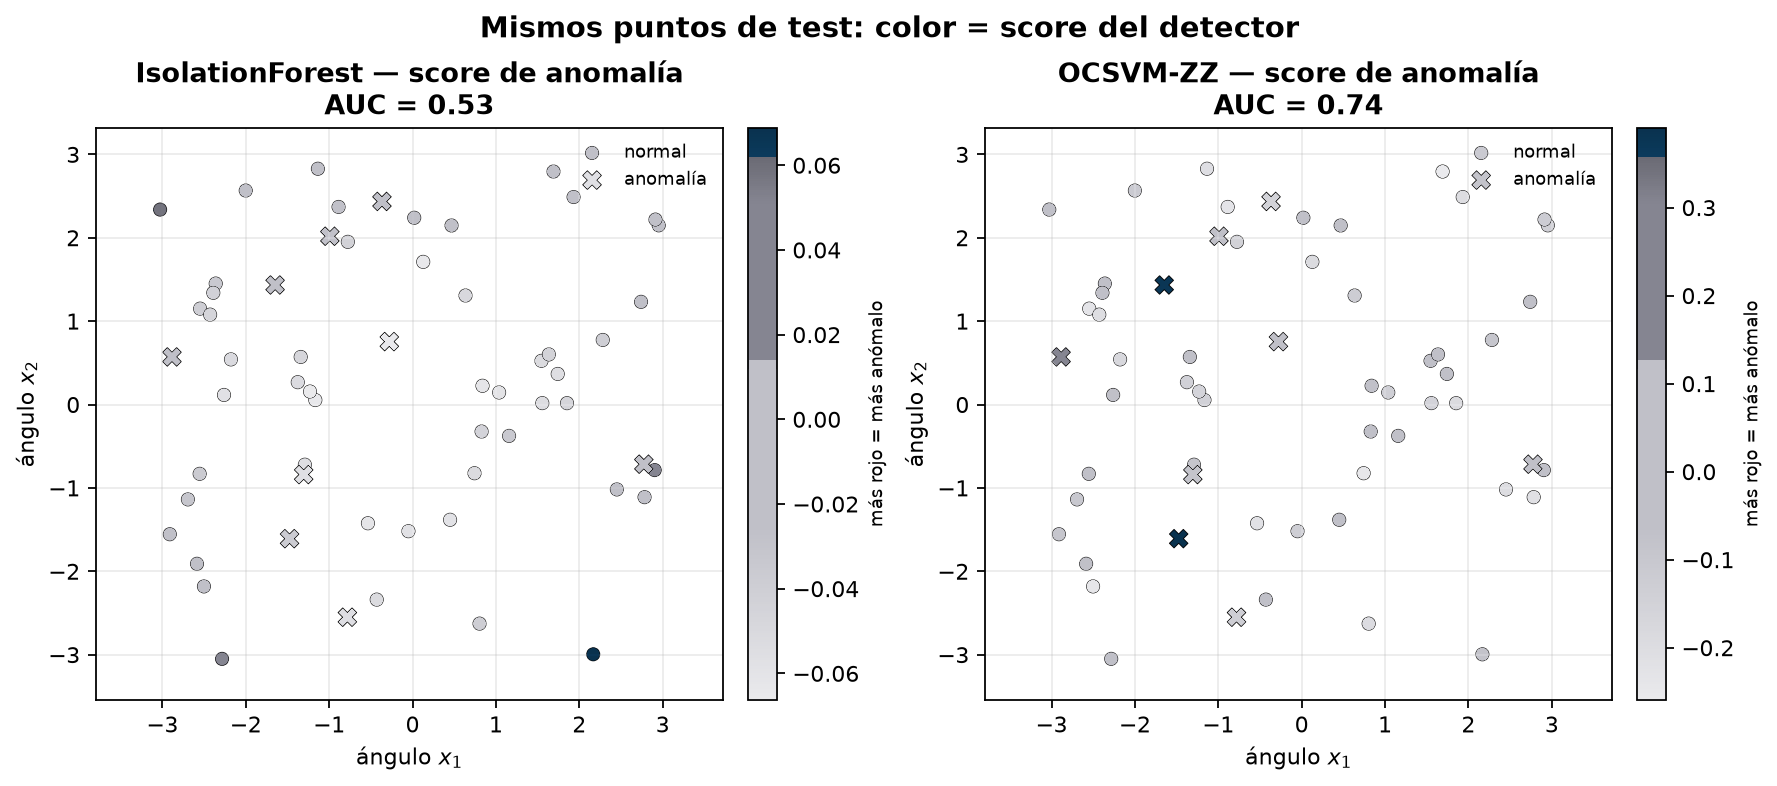
\includegraphics[width=0.98\textwidth]{Imagenes/zz_phase_scores_if_vs_zz.png}
\caption{Mismos puntos de test en \texttt{zz\_phase}: color = score de anomalía. IsolationForest obtiene AUC~$\approx 0.53$ (casi azar) y marca bordes de la nube; OCSVM-ZZ obtiene AUC~$\approx 0.74$ en este split ilustrativo (media multi-repeat $0.864$).}
\label{fig:anomaly_scores}
\end{figure}

\paragraph{Interpretación.}
La ventaja en anomalías aparece cuando lo ``raro'' \emph{no} es estar lejos, sino pertenecer a otra estructura accesible por el \textbf{feature map alineado} con el generador (aquí, fase del mapa ZZ validado empíricamente). Un mapa distinto (Pauli, IQP, \ldots) definiría otra familia de novedades beneficiadas. En tablas de práctica con spikes lejanos, IsolationForest es suficiente y más barato. El Caso~8 refuerza el mensaje transversal: el módulo cuántico es una \textbf{herramienta selectiva}, activada tras diagnóstico de alineación ($\mathcal{Q}_{\mathrm{rob}}$ / tipo de anomalía), no un sustituto por defecto de IsolationForest ni un atajo hacia ``detección de fraude cuántica''.

% =====================================================================
\section{Caso de uso 9: Forecasting one-step por lags}
\label{sec:eval_timeseries}
% =====================================================================

Los resultados de \texttt{qml\_v2.timeseries} (5 repeticiones, división temporal 70/30; Figura~\ref{fig:ts_mae}) confirman el patrón de alineación en el dominio secuencial (Tabla~\ref{tab:timeseries_dev}).

\begin{figure}[ht]
\centering
\includegraphics[width=\textwidth]{../POCs/data/output/figures/12_series_mae.png}
\caption{MAE en test (media $\pm$ desviación sobre 5 repeticiones) del Caso~9. Azul: QK-SVR-ZZ; gris oscuro: clásicos con los mismos lags (Tabla~A); gris claro: clásicos con variables adicionales (Tabla~B, marcados con *). Líneas horizontales: media del entrenamiento (discontinua) y persistencia (punteada). Fuente: \texttt{fair\_timeseries\_*.csv}, Notebook~12.}
\label{fig:ts_mae}
\end{figure}

\begin{itemize}
  \item \texttt{zz\_lag}: QK-SVR-ZZ MAE $0.056\pm0.007$ ($R^2=0.98$) frente a Ridge $0.414$, SVR-RBF $0.435$ y Gradient Boosting $0.465$; la media del entrenamiento da $0.404$, de modo que los clásicos no mejoran el predictor trivial. Ventaja por construcción: el target es $\langle ZZ\rangle$ de la ventana.
  \item \texttt{sine}: SVR-RBF $0.260$ y Ridge $0.266$ frente a QK-SVR $0.662$, que coincide con la media del entrenamiento ($0.658$). Con las variables de la Tabla~B los clásicos mejoran ligeramente ($0.244$).
  \item \texttt{skg\_speed}: Ridge $2.80\pm0.63$ frente a QK-SVR $13.59\pm5.68$ (media del entrenamiento: $13.61$). Ridge queda al nivel de la persistencia ($2.75$); con las variables de la Tabla~B el mejor clásico es Gradient Boosting ($3.24$), peor que Ridge con solo 2 lags.
\end{itemize}

\paragraph{Interpretación.}
La ventaja no es ``usar un kernel cuántico en series temporales'', sino alinear el generador del target con el feature map. Fuera del régimen nativo, el kernel ZZ con 2 qubits y $\varepsilon=0.1$ obtiene el mismo MAE que un predictor de la media del entrenamiento, es decir, no extrae señal de los lags. En la serie SKG, con solo 138 ventanas por corredor, ni siquiera los clásicos superan de forma clara a la persistencia, por lo que el valor operativo reside en el modelo lineal sobre lags y no en kernels más expresivos. ZZ es el mapa del corpus; un mapa distinto beneficiaría otra familia de series.

% =====================================================================
\section{Síntesis comparativa y discusión general}
% =====================================================================

La Tabla~\ref{tab:sintesis} sintetiza los resultados principales del estudio comparativo.

\begin{table}[ht]
\centering
\small
\setlength{\tabcolsep}{4pt}
\begin{tabular}{>{\centering\arraybackslash}p{0.7cm}>{\raggedright\arraybackslash}p{2.4cm}>{\centering\arraybackslash}p{2.5cm}>{\centering\arraybackslash}p{2.5cm}>{\centering\arraybackslash}p{2.5cm}}
\hline
\textbf{CU} & \textbf{Algoritmo cuántico} & \textbf{Cuántico-nativo} & \textbf{SKG} & \textbf{Referencia} \\
\hline
1 & QSVM & \textbf{+38.3 pp} & $-$4.5 pp & $-$3.8 pp \\
2 & QK-SVR & \textbf{$+0.965\,\Delta R^2$} & $-0.562\,\Delta R^2$ & $-0.928\,\Delta R^2$ \\
3 & QAOA ($p=1$) & \multicolumn{3}{>{\centering\arraybackslash}p{8.0cm}}{Iguala al óptimo exacto en 5/5 instancias; sin ventaja (coste idéntico)} \\
4 & VQE/QAOA & \multicolumn{3}{>{\centering\arraybackslash}p{8.0cm}}{Óptimo en 6/10 semillas (QAOA) y 3/10 (VQE) con penalización 10; Greedy y fuerza bruta, siempre ($-40$ pp)} \\
5 & QAOA TSP & \multicolumn{2}{c}{empate óptimo vs NN+2-opt ($n=4$)} & Euclidean gap~$0$ \\
6 & QSVM (umbral) & $+8.9$ pp ($n=150$, una partición) & $-4.0$ pp (clásico) & $-3.8$ pp vs GB (clásico) \\
7 & QAOA MDS ($p=3$) & \multicolumn{3}{>{\centering\arraybackslash}p{8.0cm}}{Red de 6 nodos: empate con ILP ($0$ pp); ER $n=6$--$15$: $-60$ pp de instancias con MDS óptimo (2/5 frente a 5/5)} \\
8 & OCSVM-ZZ & \textbf{+31.2 pp AUC} (\texttt{zz\_phase}) & $-29.9$ pp (inyectado) & $-29.1$ pp (moons), $-50.8$ pp (blobs) \\
9 & QK-SVR lags & \textbf{+86.6\% MAE} (\texttt{zz\_lag}) & $-385.6\%$ (\texttt{skg\_speed}) & $-154.9\%$ (\texttt{sine}) \\
\hline
\end{tabular}
\caption{Síntesis cuántico vs clásico, generada por \texttt{scripts/sintesis\_resultados.py} a partir de las salidas ejecutadas. Positivo = favorece al método cuántico; unidades: pp de exactitud (CU1, CU6), $\Delta R^2$ (CU2), pp de AUC (CU8) y mejora relativa del MAE (CU9). Negrita = ventaja sobre el mejor clásico. En kernels, la ventaja aparece \textbf{solo} en el régimen cuántico-nativo (datos generados por el propio mapa); en SKG y Telco gana GB/RF (Telco $-3.8$~pp frente a Gradient Boosting). Los Casos~1, 2 y~6 usan una sola partición con 45--60 puntos de test (granularidad de $\pm2.2$~pp).}
\label{tab:sintesis}
\end{table}

\begin{figure}[!htbp]
\centering
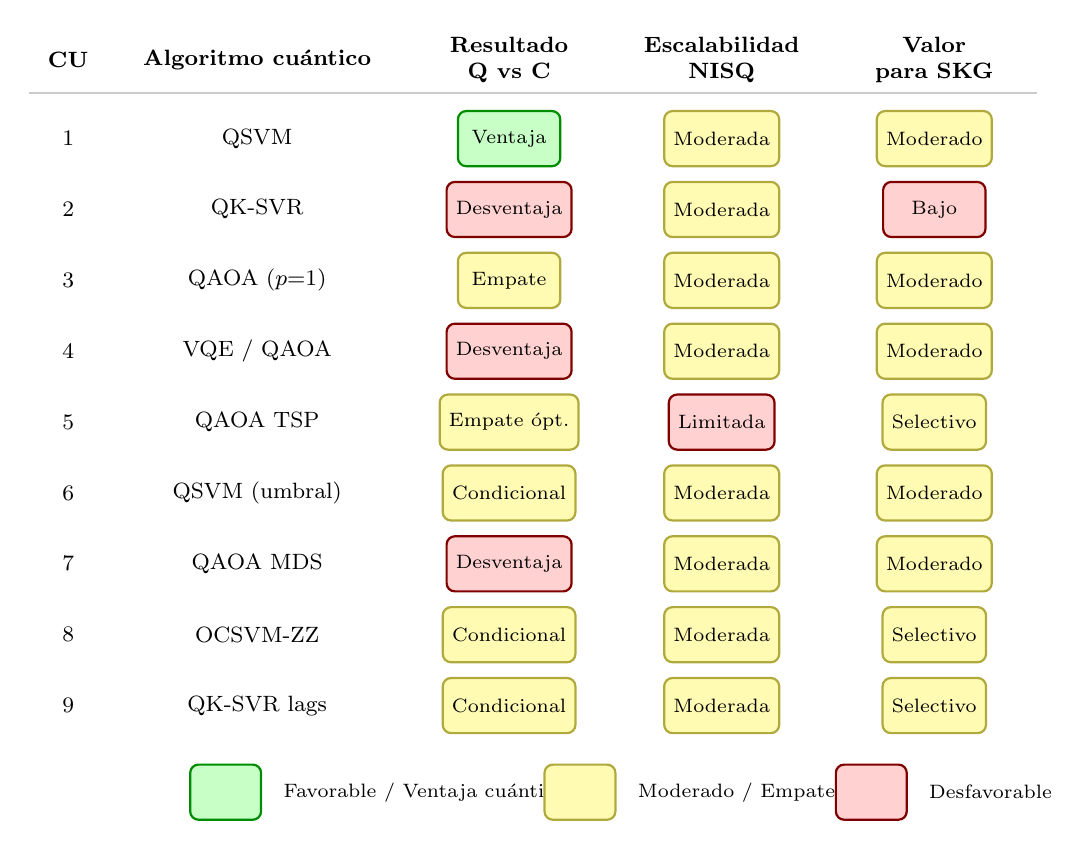
\begin{tikzpicture}[font=\small, thick,
    bg/.style={rectangle, rounded corners=3pt, minimum width=1.3cm, minimum height=0.7cm, align=center},
    verde/.style={bg, fill=green!22, draw=green!55!black},
    amarillo/.style={bg, fill=yellow!30, draw=yellow!65!black},
    rojo/.style={bg, fill=red!18, draw=red!50!black},
    header/.style={font=\bfseries\footnotesize, align=center}]

  % Columnas: x = 0(CU), 2.2(Algoritmo), 5.5(Resultado), 8.2(Escala NISQ), 10.9(Valor SKG)
  \node[header] at (0,    0) {CU};
  \node[header] at (2.4,  0) {Algoritmo cuántico};
  \node[header] at (5.6,  0) {Resultado\\ Q vs C};
  \node[header] at (8.3,  0) {Escalabilidad\\ NISQ};
  \node[header] at (11.0, 0) {Valor\\ para SKG};

  \draw[gray!40, thick] (-0.5, -0.42) -- (12.3, -0.42);

  % Fila 1 – CU1
  \node[font=\footnotesize] at (0,    -1.0) {1};
  \node[font=\footnotesize, align=left] at (2.4, -1.0) {QSVM};
  \node[verde]    at (5.6,  -1.0) {\scriptsize Ventaja};
  \node[amarillo] at (8.3,  -1.0) {\scriptsize Moderada};
  \node[amarillo] at (11.0, -1.0) {\scriptsize Moderado};

  % Fila 2 – CU2
  \node[font=\footnotesize] at (0,    -1.9) {2};
  \node[font=\footnotesize, align=left] at (2.4, -1.9) {QK-SVR};
  \node[rojo]     at (5.6,  -1.9) {\scriptsize Desventaja};
  \node[amarillo] at (8.3,  -1.9) {\scriptsize Moderada};
  \node[rojo]     at (11.0, -1.9) {\scriptsize Bajo};

  % Fila 3 – CU3
  \node[font=\footnotesize] at (0,    -2.8) {3};
  \node[font=\footnotesize, align=left] at (2.4, -2.8) {QAOA ($p{=}1$)};
  \node[amarillo] at (5.6,  -2.8) {\scriptsize Empate};
  \node[amarillo] at (8.3,  -2.8) {\scriptsize Moderada};
  \node[amarillo] at (11.0, -2.8) {\scriptsize Moderado};

  % Fila 4 – CU4
  \node[font=\footnotesize] at (0,    -3.7) {4};
  \node[font=\footnotesize, align=left] at (2.4, -3.7) {VQE / QAOA};
  \node[rojo]     at (5.6,  -3.7) {\scriptsize Desventaja};
  \node[amarillo] at (8.3,  -3.7) {\scriptsize Moderada};
  \node[amarillo] at (11.0, -3.7) {\scriptsize Moderado};

  % Fila 5 – CU5
  \node[font=\footnotesize] at (0,    -4.6) {5};
  \node[font=\footnotesize, align=left] at (2.4, -4.6) {QAOA TSP};
  \node[amarillo] at (5.6,  -4.6) {\scriptsize Empate ópt.};
  \node[rojo]     at (8.3,  -4.6) {\scriptsize Limitada};
  \node[amarillo] at (11.0, -4.6) {\scriptsize Selectivo};

  % Fila 6 – CU6
  \node[font=\footnotesize] at (0,    -5.5) {6};
  \node[font=\footnotesize, align=left] at (2.4, -5.5) {QSVM (umbral)};
  \node[amarillo] at (5.6,  -5.5) {\scriptsize Condicional};
  \node[amarillo] at (8.3,  -5.5) {\scriptsize Moderada};
  \node[amarillo] at (11.0, -5.5) {\scriptsize Moderado};

  % Fila 7 – CU7
  \node[font=\footnotesize] at (0,    -6.4) {7};
  \node[font=\footnotesize, align=left] at (2.4, -6.4) {QAOA MDS};
  \node[rojo]     at (5.6,  -6.4) {\scriptsize Desventaja};
  \node[amarillo] at (8.3,  -6.4) {\scriptsize Moderada};
  \node[amarillo] at (11.0, -6.4) {\scriptsize Moderado};

  % Fila 8 – CU8
  \node[font=\footnotesize] at (0,    -7.3) {8};
  \node[font=\footnotesize, align=left] at (2.4, -7.3) {OCSVM-ZZ};
  \node[amarillo] at (5.6,  -7.3) {\scriptsize Condicional};
  \node[amarillo] at (8.3,  -7.3) {\scriptsize Moderada};
  \node[amarillo] at (11.0, -7.3) {\scriptsize Selectivo};

  % Fila 9 – CU9
  \node[font=\footnotesize] at (0,    -8.2) {9};
  \node[font=\footnotesize, align=left] at (2.4, -8.2) {QK-SVR lags};
  \node[amarillo] at (5.6,  -8.2) {\scriptsize Condicional};
  \node[amarillo] at (8.3,  -8.2) {\scriptsize Moderada};
  \node[amarillo] at (11.0, -8.2) {\scriptsize Selectivo};

  % Leyenda
  \node[verde,    minimum width=0.9cm] (lg) at (2.0, -9.3) {};
  \node[right=4pt, font=\scriptsize] at (lg.east) {Favorable / Ventaja cuántica};
  \node[amarillo, minimum width=0.9cm] (ly) at (6.5, -9.3) {};
  \node[right=4pt, font=\scriptsize] at (ly.east) {Moderado / Empate};
  \node[rojo,     minimum width=0.9cm] (lr) at (10.2, -9.3) {};
  \node[right=4pt, font=\scriptsize] at (lr.east) {Desfavorable};

\end{tikzpicture}
\caption{Semáforo de resultados por caso de uso. Azul = favorable; gris claro = moderado, empate o condicional; gris = desfavorable. La columna ``Resultado'' se deriva de la Tabla~\ref{tab:sintesis}; ``Escalabilidad NISQ'' y ``Valor para SKG'' son valoraciones cualitativas del autor, no mediciones. Los Casos~8 y~9 son condicionales: hay ventaja cuando novedad o target están alineados con el feature map (aquí ZZ). Caso~7: empate en la red de 6 nodos y $-60$~pp de instancias con MDS óptimo en los grafos ER.}
\label{fig:semaforo_resultados}
\end{figure}

\clearpage
\begin{figure}[!htbp]
\centering
\includegraphics[width=0.97\textwidth]{../POCs/data/output/figures/07_dashboard_ventaja_cuantica.png}
\caption{Dashboard de los nueve casos de uso, generado a partir de \texttt{07\_sintesis\_resultados.csv}. Cada panel usa la unidad de su caso (pp de exactitud, $\Delta R^2\times100$, \% de coste, pp de AUC, \% de MAE o pp de instancias con MDS óptimo); positivo favorece al método cuántico. Azul = ventaja cuántica; gris = clásico superior; gris claro = empate. Coherente con la Tabla~\ref{tab:sintesis}.}
\label{fig:dashboard_sintesis}
\end{figure}

\begin{figure}[!htbp]
\centering
\includegraphics[width=0.90\textwidth]{../POCs/data/output/figures/07_heatmap_ventaja_por_dominio.png}
\caption{Mapa de calor de la ventaja cuántica sobre el mejor clásico por caso de uso y tipo de dataset, con la unidad indicada en cada fila; el color se satura en $\pm80$ y la anotación conserva el valor real. Las celdas azules aparecen solo con alineación feature map--generador (Casos~1, 2, 6, 8 y~9 en datos nativos). Las celdas grises reflejan dominio clásico. Los Casos~3, 4 y~5 no distinguen tipo de dataset y se sitúan en la columna de referencia; el Caso~7 se mide en pp de instancias con MDS óptimo frente a ILP/Greedy y se sitúa en la columna de referencia.}
\label{fig:heatmap_ventaja_body}
\end{figure}

\begin{figure}[!htbp]
\centering
\includegraphics[width=0.95\textwidth]{../POCs/data/output/figures/07_grover_benchmark.png}
\caption{Conteo teórico de operaciones del algoritmo de Grover ($\lfloor\pi\sqrt{N}/4\rfloor$ iteraciones) frente a la búsqueda clásica no estructurada ($N$ comparaciones) en función del tamaño del espacio de búsqueda $N$. Es una ilustración analítica: no se ejecutó Grover ni se midió tiempo, y no incluye el coste del oráculo. La aceleración cuadrática se hace evidente a partir de $N \approx 10^3$, ilustrando el tipo de ventaja estructural que la computación cuántica puede aportar a problemas de búsqueda y optimización.}
\label{fig:grover_benchmark}
\end{figure}

\begin{figure}[!htbp]
\centering
\includegraphics[width=0.95\textwidth]{../POCs/data/output/figures/07_paralelismo_cuantico.png}
\caption{Superposición de $n$ qubits tras aplicar Hadamard a $|0\rangle^{\otimes n}$: el vector de estado tiene $2^n$ amplitudes iguales ($1/2^n$ de probabilidad cada una). Que el espacio de Hilbert crezca exponencialmente no implica que el computador cuántico evalúe $2^n$ casos a la vez: una medición devuelve un único resultado, y la ventaja de algoritmos como Grover o Shor proviene de la interferencia, no del mero paralelismo.}
\label{fig:paralelismo_cuantico}
\end{figure}

\subsection{Patrones transversales}

Los resultados evidencian tres patrones transversales que son coherentes con el estado actual de la teoría y la tecnología cuántica:

\begin{enumerate}
  \item \textbf{La ventaja cuántica requiere alineación dato--feature map}: La ventaja observada en datos nativos es coherente con \cite{huang2021}: el feature map (ZZ u otro) debe estar alineado con el generador; ZZ es el mapa validado empíricamente en este TFM, no un monopolio. En datos reales sin esa alineación, Gradient Boosting y Random Forest mantienen su superioridad.

  \item \textbf{El cuello de botella es la escala}: En todos los casos, la principal limitación práctica del enfoque cuántico no es la calidad del algoritmo sino el coste cuadrático del kernel ($O(n^2)$) y el número de qubits disponibles \citep{haug2023, cerezo2021}. Esta limitación es una función del hardware actual, no del algoritmo en sí.

  \item \textbf{Los resultados negativos son informativos}: Los casos donde el QSVM o el QK-SVR son inferiores a los clásicos en datos reales no son fracasos experimentales, sino resultados metodológicamente valiosos que delimitan el dominio de aplicabilidad. El Caso~8 añade el mismo matiz en one-class: OCSVM-ZZ no sustituye IsolationForest salvo cuando la novedad está alineada con el mapa (aquí \texttt{zz\_phase}), no cuando es geométrica clásica.
\end{enumerate}

\subsection{Implicaciones para la adopción empresarial}

Desde la perspectiva de SKG Tecnología, los resultados sugieren que la integración de algoritmos cuánticos en los sistemas de gestión de movilidad urbana requiere dos condiciones previas: (i) hardware cuántico con mayor número de qubits lógicos y menor tasa de error \citep{preskill2018, cerezo2023}, para operar sobre más features sin reducción dimensional, y (ii) ingeniería de features específica que alinee la representación de los datos con las estructuras geométricas accesibles por los kernels cuánticos \citep{huang2021}. En el corto plazo (horizonte 2--5 años), el valor más realista de la computación cuántica para SKG reside en los algoritmos de optimización combinatoria (QAOA, VQE) para problemas de asignación de recursos, aunque en los casos medidos aquí (3, 4, 5 y 7) ningún solver cuántico ha superado a los exactos \citep{farhi2014}.

El hilo conductor de los nueve casos de uso es precisamente la demostración de que los algoritmos cuánticos no necesitan reemplazar a los clásicos para ser útiles: basta con que resuelvan de forma más eficaz la parte del problema que es intratable para la computación clásica \citep{biamonte2017}. El Caso~7 lo ilustra de forma paradigmática: aplicar QAOA al conjunto dominante mínimo ---un problema NP-difícil--- y conectarlo con un optimizador clásico COBYLA a través de una interfaz mínima es exactamente el patrón con el que la computación cuántica puede integrarse en entornos productivos reales \citep{farhi2014}. El prototipo de arquitectura híbrida desarrollado en la Sección~\ref{sec:prototipo_hibrido} del Capítulo~\ref{cap:metodologia} formaliza este patrón y define los criterios de activación del módulo cuántico según el tipo de problema.

\subsection{Resultados adicionales y visualización}

El análisis de escalabilidad del caso~1 se sintetiza en la Figura~\ref{fig:escala_clasificacion}: ventaja positiva en $n \in [30, 180]$ (10 repeticiones por tamaño) \textbf{solo} en el régimen cuántico-nativo. La geometría de kernel se reporta vía los indicadores tabulares del Capítulo~\ref{cap:investigacion_original} ($\Delta A$, $d_F$, $\Delta H$); no se usan heatmaps regenerados a posteriori (las matrices $K$ no se exportaron a artefactos). $\mathcal{Q}>0$ vs.\ un baseline débil no basta como veredicto operativo.

